\documentclass[12pt]{article}

\usepackage[top=0.75in,bottom=0.75in,left=0.5in,right=0.5in]{geometry}
\usepackage{amsmath,amssymb,multirow,graphicx,multirow}

\newcommand{\bee}[1]{\begin{equation} #1 \end{equation}}
\newcommand{\baa}[1]{\begin{eqnarray} #1 \end{eqnarray}}
\newcommand{\bees}[1]{\begin{equation*} #1 \end{equation*}}
\newcommand{\baas}[1]{\begin{eqnarray*} #1 \end{eqnarray*}}

\newcommand{\pd}[2]{\ensuremath{\frac{\partial #1}{\partial #2}}}
\newcommand{\dd}[2]{\ensuremath{\frac{d #1}{d #2}}}

\newcommand{\bx}{{\mathbf x}}
\newcommand{\ba}{{\mathbf a}}
\newcommand{\bl}{{\pmb \ell}}
\newcommand{\bu}{{\mathbf u}}
\newcommand{\bv}{{\mathbf v}}
\newcommand{\bq}{{\mathbf q}}
\newcommand{\bp}{{\mathbf p}}
\newcommand{\bg}{{\mathbf g}}
\newcommand{\ff}{{\mathbf f}}
\newcommand{\bS}{{\mathbf S}}
\newcommand{\bI}{{\mathbf I}}
\newcommand{\bA}{{\mathbf A}}
\newcommand{\bG}{{\mathbf G}}
\newcommand{\bF}{{\mathbf F}}
\newcommand{\bP}{{\mathbf P}}
\newcommand{\bQ}{{\mathbf Q}}

\newcommand{\eps}{\epsilon}
\newcommand{\Ge}{\bG_\eps}
\newcommand{\Gec}{G_\eps}


\begin{document}
	
	\section*{Introduction}
	
	This set of notes explores the addition of various incompressible background flows to the regularized Lagrangian formulation of Stokes-OB flow. My main observations are the following:
	
	\begin{enumerate}
		\item Both a background flow and its Eulerian gradient are needed for the calculations.
		\item Background flows that are chosen must satisfy the Stokes equations. This means they must not only be incompressible, but also have a potential flow (pressure gradient) to balance the Laplacian.
		\item The Lagrangian method is suitable only for flows in which the deviation of the stress from a background level is compact, or approximately so, in all directions. For example, a flow that creates constant stress in one direction and decaying stress away from zero in the other direction can be modeled using the Lagrangian approach.
		\item The four roll mill flow introduced below does not have compact stress in any direction and cannot be accurately modeled with our method. [*Unless* maybe modeling a full block of all four cells would be accurate enough. I have not tried this. I would want to interpolate back to the original grid for regridding.]
		\item The linearized four roll mill flow provides two exact solutions to the Stokes-OB flow that can be modeled, one of which is independent of both spatial variables and one that depends on $y$. These can be used to verify, at least in a limited fashion, the accuracy of the implementation.
		\item The search for other exact solutions with spatially varying but rapidly decaying (approximately compact) flows was not successful.
	\end{enumerate}
	
	\section*{Lagrangian four roll mill flow}
	
	A four roll mill has a background velocity field of 
	%
	\[ \bu_b = U(\sin x \cos y, -\cos x \sin y), \]
	%
	where $U$ is a constant. This causes hyperbolic stagnation points in the flow at each point $(k\pi,n\pi)$, where $k$ and $n$ are integers. 
	
	Recall that the general regularized Lagrangian formulation is given by
	%
	\baas{
	\bv &=& \int_{\Omega(0)} \Ge(\bl(\ba,t) - \bl(\ba',t)) \left( \beta \nabla_{a'} \cdot \bP(\ba',t) + \ff(\bl(\ba',t),t) \right) d\ba' \\
	\pd{\bP}{t} &=& \left(\nabla_a \bv \right)\bF^{-1}\bP - Wi^{-1}\left( \bP - \bF^{-T} \right),
	}
	%
	where $\bv$ is the Lagrangian velocity $\partial \bl / \partial t$, $F$ is the deformation matrix, and $\bP = \bS \bF^{-T}$ where $\bS$ is the polymer stress tensor (see the Model Derivation notes for more detail). For the four roll mill case, we do not have body forces $\ff$, but we do have a background velocity that must be added to each Lagrangian point. This gives us an additional term in both of the equations as follows:
	%
	\begin{align}
		 \frac{\partial \bl}{\partial t} &= \bu_b(\bl(\ba,t)) + \int_{\Omega(0)} \Ge(\bl(\ba,t) - \bl(\ba',t)) \left( \beta \nabla_{a'} \cdot \bP(\ba',t) \right) d\ba'  \label{OBw/vel1}\\
		\pd{\bP}{t} &= \left(\nabla_a \bu_b(\bl(\ba,t)) \right)\bF^{-1}\bP + \left(\int_{\Omega(0)} \Ge^D(\bl(\ba,t) - \bl(\ba',t)) \left( \beta \nabla_{a'} \cdot \bP(\ba',t) \right) d\ba' \right)\bF^{-1}\bP - Wi^{-1}\left( \bP - \bF^{-T} \right), \label{OBw/vel2}
	\end{align}
	%
	where the derivation of the integral term in the second equation is in the Model Derivation notes. The first term in the second equation can be simplified:
	%
	\begin{align*}
		\left(\nabla_a \bu_b(\bl(\ba,t)) \right)\bF^{-1}\bP &= \left(\nabla_x \bu_b(\bx) \bF \right)\bF^{-1}\bP \\ 
		&= \left(\nabla_x \bu_b \right)\bP, 
	\end{align*}
	%
	where
	%
	\[ \nabla_x \bu_b = U \begin{pmatrix} \cos x \cos y & -\sin x \sin y \\ \sin x \sin y & -\cos x \cos y \end{pmatrix} \]
	%
	for the four roll mill flow.
	
	\section*{Linearization}
	
	If we linearize near the stagnation point $(0,0)$, we see flow like 
	%
	\begin{align} 
		\bu_b &= U(x, -y) \label{linflow} \\
		\nabla_x \bu_b &= U\begin{pmatrix} 1 & 0 \\ 0 & -1\end{pmatrix}. \label{gradlinflow}
	\end{align}
	%
	If we assume that $U>0$, then the flow stretches the fluid in the $x$-direction near $(0,0)$, and the component of the stress tensor that is largest should be the upper left component $S_{11}$. 
	
		
	\section*{Exact solution with constant initial conditions}
	
	For validation purposes, we would like an exact solution to Eqs.~\eqref{OBw/vel1}-\eqref{OBw/vel2}. To find such a solution, we will consider the linearization of the four roll mill velocity near the stagnation point $(0,0)$ in Eqs.~\eqref{linflow}-\eqref{gradlinflow}. We substitute this flow into Eq.~\eqref{OBw/vel2} \textbf{assuming for the moment that $\beta =0$.} That is, we are solving for the first term in a regular perturbation expansion with respect to $\beta$, which results in the equations:
	%
	\begin{align*}
		 \bu_b(x,y) &= \dot{\bx} = U(x, -y)  \\
		\frac{\partial \bl}{\partial t} &= \bv = \bu_b(\bl(\ba,t)) \\		
		\pd{\bP}{t} &= \left(\nabla_x \bu \right)\bP - Wi^{-1}\left( \bP - \bF^{-T} \right) \\
		&= \begin{pmatrix} 1 & 0 \\ 0 & -1\end{pmatrix}\bP - Wi^{-1}\left( \bP - \bF^{-T} \right)
	\end{align*}	
	%
	The first equation is in Eulerian coordinates and the last two are Eqs.~\eqref{OBw/vel1}-\eqref{OBw/vel2} with $\beta = 0$. It is easily seen that $x = a e^{Ut}$ and $y = b e^{-Ut}$, where $(a,b)$ are the initial locations of the points and therefore are the Lagrangian coordinates in the flow map: 
	%
	\begin{align*}
		\bl &= (a e^{Ut}, b e^{-Ut}),
	\end{align*}	
	%	
	leading to a deformation matrix of
	%
	\begin{align*}
		\bF = \left(\nabla_a \bl \right) &= \begin{pmatrix} e^{Ut} & 0 \\ 0 & e^{-Ut} \end{pmatrix} \\
		\Rightarrow \bF^{-1} &= \begin{pmatrix} e^{-Ut} & 0 \\ 0 & e^{Ut} \end{pmatrix} = \bF^{-T}.
	\end{align*}	
	%
	Notice that all these matrices are independent of spatial variables.
	
	Now we solve for the Lagrangian stress $\bP$.
	%
	\begin{align*}
		\pd{\bP}{t} &= U\begin{pmatrix} 1 & 0 \\ 0 & -1\end{pmatrix}\bP - Wi^{-1}\left( \bP - \begin{pmatrix} e^{-Ut} & 0 \\ 0 & e^{Ut} \end{pmatrix} \right),
	\end{align*}	
	%
	which is a system of equations for each of the components of $\bP$:
	%
	\begin{align*}
		\pd{P_{11}}{t} &= UP_{11} - Wi^{-1}\left( P_{11} - e^{-Ut} \right) \\
		\pd{P_{12}}{t} &= - Wi^{-1}P_{12} \\
		\pd{P_{21}}{t} &= - Wi^{-1}P_{21} \\
		\pd{P_{22}}{t} &= -UP_{22} - Wi^{-1}\left( P_{22} - e^{Ut} \right),
	\end{align*}	
	%
	with an initial condition of no stress everywhere in the domain:
	%
	\begin{align*}
		\bP(\bl,0) &= \begin{pmatrix} 1 & 0 \\ 0 & 1\end{pmatrix}.
	\end{align*}	
	%
	Then $P_{12} = P_{12}(0)e^{-Wi^{-1}t} = 0$, and likewise $P_{21} = 0$, so that $\bP$ is a diagonal matrix. For the diagonal elements, we have
	%
	\begin{align*}
		\pd{P_{11}}{t} - \left(U- Wi^{-1}\right)P_{11} &= Wi^{-1}e^{-Ut} \\
		\pd{P_{22}}{t} + \left(U+ Wi^{-1}\right)P_{22} &= Wi^{-1}e^{Ut}.
	\end{align*}	
	%
	The homogeneous solutions for the diagonal elements are 
	%
	\begin{align*}
		P_{11}^H = C_1 e^{\left(U- Wi^{-1}\right)t} \\
		P_{22}^H = C_2 e^{-\left(U+ Wi^{-1}\right)t}.
	\end{align*}	
	%
	The particular solutions are of the form $Q_1 e^{-Ut}$ and $Q_2 e^{Ut}$, and solving for the unknown constants, we find
	%
	\begin{align*}
		-Q_1 U - Q_1\left(U- Wi^{-1}\right) &= Wi^{-1} \\
		\Rightarrow Q_1 = \frac{Wi^{-1} }{Wi^{-1} -2U} &= \frac{1 }{1 -2WiU} \\
		Q_2 U + Q_2\left(U+ Wi^{-1}\right) &= Wi^{-1} \\
		\Rightarrow Q_2 = \frac{Wi^{-1} }{Wi^{-1} +2U} &= \frac{1 }{1 +2WiU}.
	\end{align*}	
	%
	So the diagonal elements are given by
	%
	\begin{align*}
		P_{11} = C_1 e^{\left(U- Wi^{-1}\right)t}  + \frac{e^{-Ut} }{1 -2WiU} \\
		P_{22} = C_2 e^{-\left(U+ Wi^{-1}\right)t} + \frac{e^{Ut} }{1 +2WiU},
	\end{align*}	
	%
	with $C_1$ and $C_2$ determined by the initial conditions:
	%
	\begin{align*}
		C_1 &= 1 - \frac{1 }{1 -2WiU} = \frac{-2WiU }{1 -2WiU}\\
		C_2 &= 1 - \frac{1 }{1 +2WiU} = \frac{2WiU }{1 -2WiU} \\
		\Rightarrow & \\
		P_{11} &= \frac{-2WiU  e^{\left(U- Wi^{-1}\right)t} + e^{-Ut} }{1 -2WiU} \\
		P_{22} &= \frac{ 2WiU  e^{-\left(U+ Wi^{-1}\right)t} + e^{Ut} }{1 +2WiU}.		
	\end{align*}	
	%
	
	The Eulerian stress may be found either by solving the analogous Eulerian equations (see the next section), or may be calculated using the formula $\bP=\bS \bF^{-T}=\bS \bF^{-1}$:
	%
	\begin{align}
		\bS &= \bP\bF \nonumber\\
		\Rightarrow & \nonumber\\
		S_{11} &= \frac{-2WiU  e^{\left(U- Wi^{-1}\right)t} + e^{-Ut} }{1 -2WiU} e^{Ut} \nonumber\\
			   &= \frac{-2WiU  e^{\left(2U- Wi^{-1}\right)t} + 1 }{1 -2WiU} \nonumber \\
		S_{22} &= \frac{ 2WiU  e^{-\left(U+ Wi^{-1}\right)t} + e^{Ut} }{1 +2WiU} e^{-Ut} \nonumber\\		
			   &= \frac{ 2WiU  e^{-\left(2U+ Wi^{-1}\right)t} + 1 }{1 +2WiU}. \label{S22soln}
	\end{align}	
	%
	Notice that the stress in both Lagrangian and Eulerian variables is completely independent of space, so that any spatial derivatives of the stress are zero. In particular, $\nabla_a \cdot \bP = \mathbf{0}$, which means that this solution is valid even when $\beta$ is nonzero. Thus we have an exact solution to Eqs.~\eqref{OBw/vel1}-\eqref{OBw/vel2} with $\bu_b = U(x,-y)$.
	
	We can make several predictions about the behavior of the numerical solution to validate our work. First remember that $U>0$. Given this assumption: 
	\begin{enumerate}
		\item The lower diagonal element of the Eulerian stress $S_{22}$ decays exponentially in time to constant value of $1/(1+2WiU)$. 
		\item $S_{11}$ will become exponentially large in time if $2U-1/Wi > 0$, which is the same condition derived in the previous section. If $2U-1/Wi < 0$, then $S_{11} \to 1/(1-2WiU)$.
		\item $P_{22}$ will always become exponentially large. 
		\item $P_{11} \to 0$ if $U - 1/Wi < 0$ (a different condition), and will grow exponentially if $U - 1/Wi > 0$.
		\item The particle paths will follow the flow map $\bl = (a e^{Ut}, b e^{-Ut})$, where $(a,b)$ denotes the initial position of a point.
		\item If the finite difference scheme is second order, then $\bF = \nabla_a \cdot \bl$ is calculated exactly, since $\bl$ is linear in $(a,b)$. So there should be no decrease in error with decreasing grid spacing $h$.
		\item Since $\nabla_a \cdot \bP = \mathbf{0}$, there should be no error contribution from the regularization in $\eps$.
		\item We can use the exact solution to identify error from the regridding scheme, since there is no $h$ dependence.
	\end{enumerate}
	
	\subsection*{Results}
	
	I ran simulations with three different Weissenberg numbers chosen to capture the three different types of behavior possible in the stresses: no exponential growth in either $S_{11}$ or $P_{11}$, exponential growth in $S_{11}$ but not $P_{11}$, and exponential growth in both $S_{11}$ and $P_{11}$. The numerical results showed these expected patterns. See Figs.~\ref{WiU}-\ref{WiU12} for the results when $dt = $ 1.e-5, $N=$ 20, and $\beta = 1/(2*Wi)$. 

	\begin{figure}[htp]
		\centering
		\begin{tabular}{cc}
			$Wi = 1.2:$ Eulerian stress $S$ & $Wi = 1.2:$ Lagrangian stress $P$ \\
			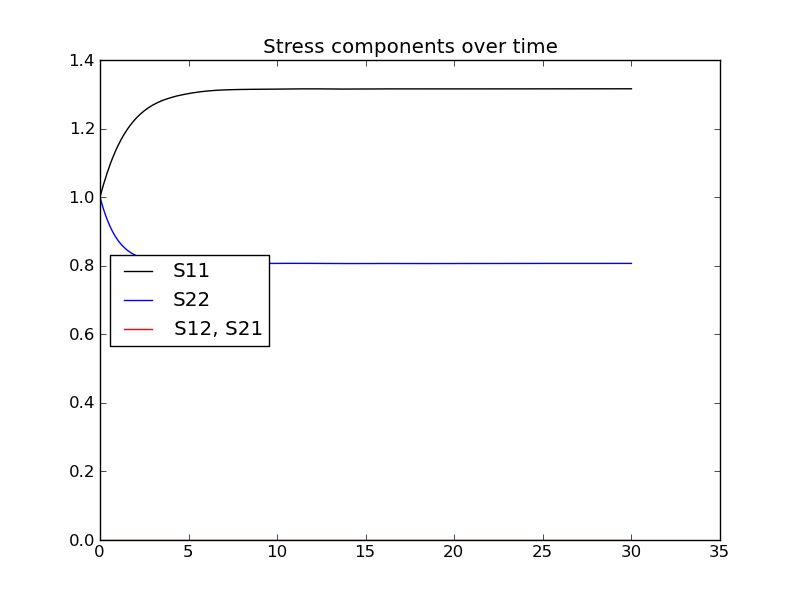
\includegraphics[width=3.0in]{Wi01_S.png} & 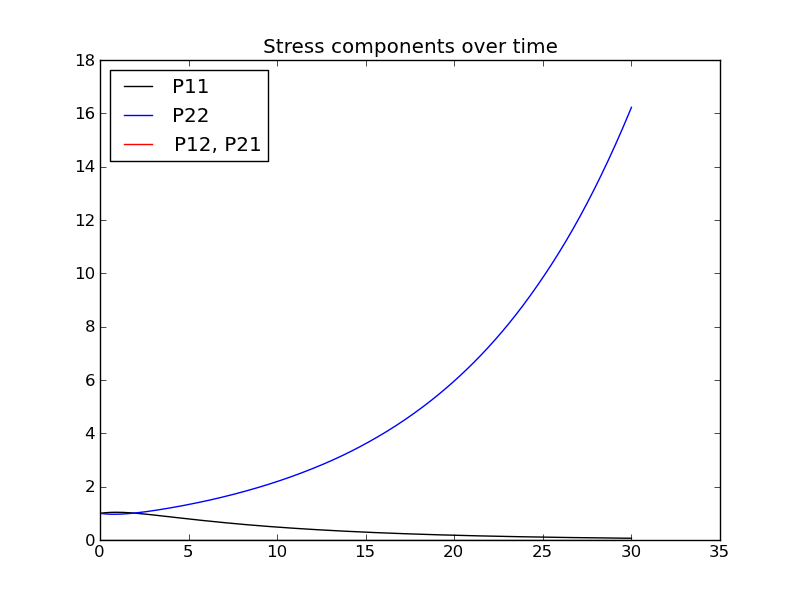
\includegraphics[width=3.0in]{Wi01_P.png} \\
			$Wi = 7.0:$ Eulerian stress $S$ & $Wi = 7.0:$ Lagrangian stress $P$ \\
			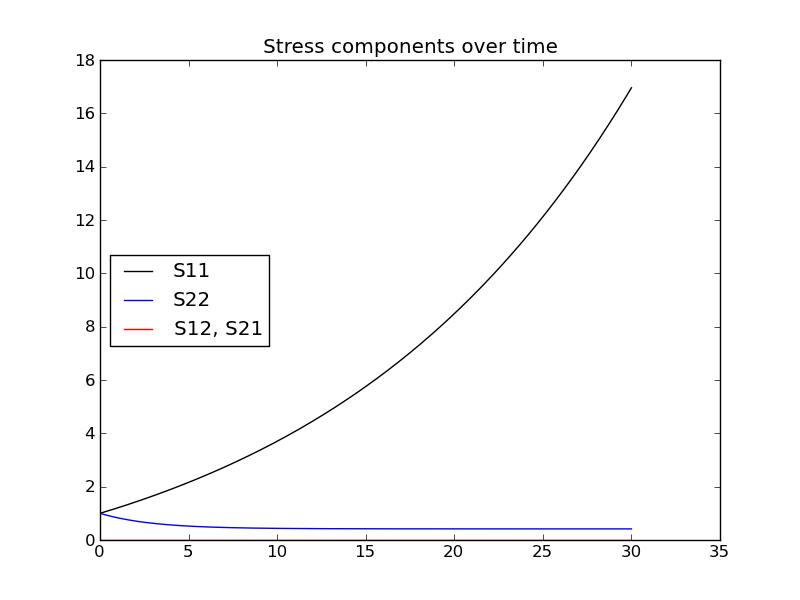
\includegraphics[width=3.0in]{Wi07_S.png} & 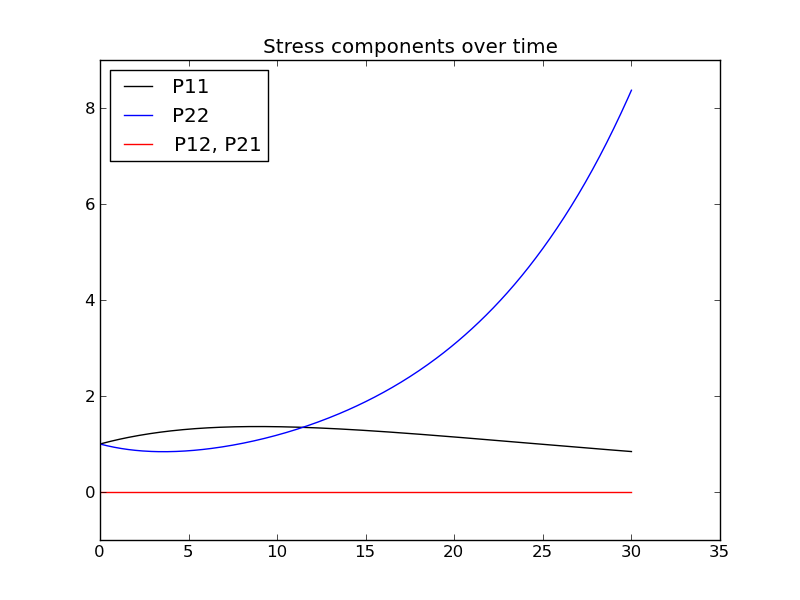
\includegraphics[width=3.0in]{Wi07_P.png} \\
		\end{tabular} 
		\caption{The behavior of stress components over time for different $Wi$.}
		\label{WiU}
	\end{figure}
	
	\begin{figure}[hbp]
		\centering
		\begin{tabular}{cc}
			$Wi = 12.0:$ Eulerian stress $S$ & $Wi = 12.0:$ Lagrangian stress $P$ \\
			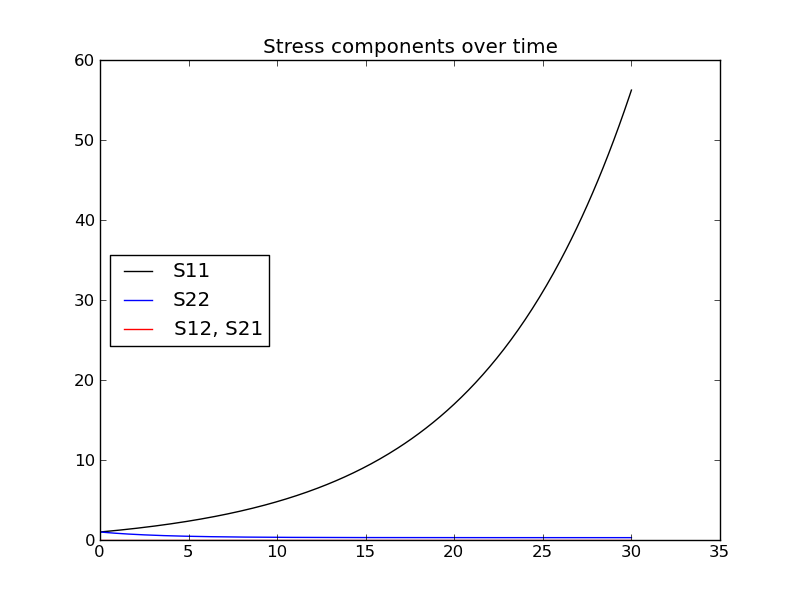
\includegraphics[width=3.0in]{Wi12_S.png} & 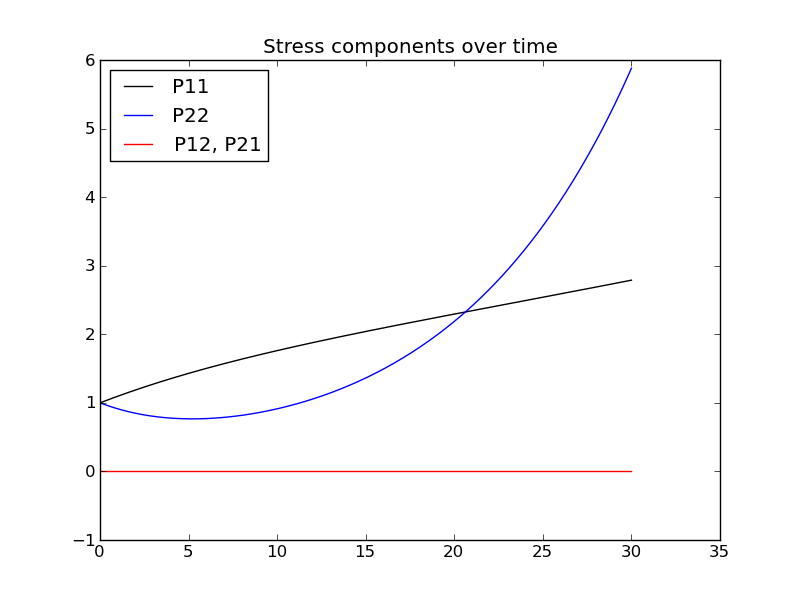
\includegraphics[width=3.0in]{Wi12_P.png} \\
			                                 \multicolumn{2}{c}{$Wi = 12.0:$ $P_{11}$ over longer time} \\
			                                 \multicolumn{2}{c}{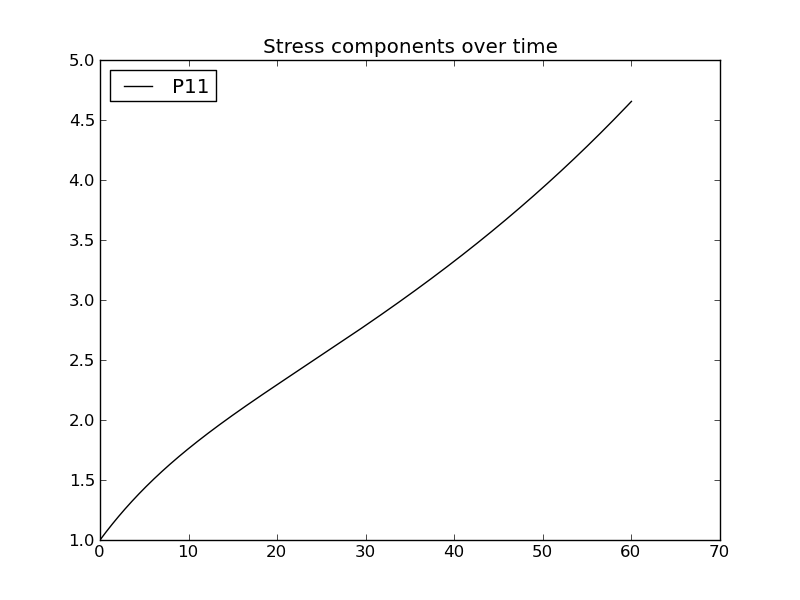
\includegraphics[width=3.0in]{Wi12_P11only.png}}
		\end{tabular} 
		\caption{The behavior of stress components over time for different $Wi$.}
		\label{WiU12}
	\end{figure}

	
	
	\subsubsection*{Relative errors when varying $Wi$, $h$, and $dt$}
	
	I ran a set of simulations that varied the time step ($dt=$ 1.e-5, 5.e-6, and 2.5e-6), number of points per side of the domain ($N=$ 20, 40, and 80) corresponding to decreasing grid spacings ($h$ = 0.025, 0.0125, and 0.00625), Weissenberg number ($Wi=$ 1.2, 7.0, and 12.0), and $\beta = 1/(2*Wi)$. In all simulations the magnitude of the extensional flow was $U=0.1$, $\eps = 0.0616$, and the final simulation time was 30. The three $Wi$ were chosen to capture the three different types of behavior possible in the stresses: no exponential growth in either $S_{11}$ or $P_{11}$, exponential growth in $S_{11}$ but not $P_{11}$, and exponential growth in both $S_{11}$ and $P_{11}$. 
	
	Relative errors in the numerical solutions were calculated using both $L_\infty$ and $L_2$ norms. Since the solution was independent of space, the relative error in the $L_2$ norm was the same as the $L_\infty$ norm, and only the latter relative errors are reported in Table~\ref{relerrs}. The relative errors are order 1.e-3, validating our solution technique. However, I was expecting the relative errors to decrease with a decreasing time step, which they do not. This is probably because I set the relative tolerance to 1.e-3 in the scipy ode solver. This solver has an adaptive step size, so no matter what time step I give it, it will iterate until it has achieved the appropriate relative tolerance. I checked this hypothesis by changing the relative tolerance to 1.e-4 for $Wi=$ 1.2 and $dt=$ 1.e-5, and the maximum relative error was 4.4e-4, supporting my conjecture.
	
	There were negligible differences (Table~\ref{diffrelerrs}) between the solutions up to time 30 for all grid spacings when $Wi = 7.0$ or 12.0. However, when $Wi = 1.2$ the similarity only held until time 15, at which point substantial differences in the relative errors emerged. I speculate that regridding might avoid these differences in the solutions. Update: I am wrong. Regridding does nothing in this case because the solutions are independent of space. See the regridding section below.
	
	\begin{table}[htp]
		\centering
		\begin{tabular}{|c|c|c|c|c|c|c|}
			\hline
			time span	& \multicolumn{3}{c}{$t\leq 15$}  &\multicolumn{3}{|c|}{$t\leq 30$} \\
			\hline
			$dt$ & $1\times10^{-5}$  & $ 5\times10^{-6}$  & $2.5\times10^{-6}$& $1\times10^{-5}$ & $5\times10^{-6}$  & $2.5\times10^{-6}$\\
			\hline
			\hline
			$Wi = 1.2$    & $1.0\times 10^{-3}$ & $1.0\times 10^{-3}$ & $2.7\times 10^{-3}$ & $2.2\times 10^{-3}$  & $3.5\times 10^{-3}$ & $2.7\times 10^{-3}$\\
			$Wi = 7.0$    & $1.8\times 10^{-3}$ & $1.3\times 10^{-3}$ & $1.4\times 10^{-3}$ & $2.0\times 10^{-3}$  & $3.1\times 10^{-3}$ & $3.0\times 10^{-3}$\\
			$Wi = 12.0$   & $2.0\times 10^{-3}$ & $1.9\times 10^{-3}$ & $1.8\times 10^{-3}$ & $5.1\times 10^{-3}$  & $2.1\times 10^{-3}$ & $4.3\times 10^{-3}$\\
			\hline
		\end{tabular}
		\caption{\textbf{Maximum relative error in stress and position over the course of the simulation.} The relative $L_\infty$ error was calculated at each time step and each grid spacing $h$ for the diagonal elements of the Eulerian and Lagrangian stresses and for the $x$ and $y$ positions of all of the particles. The table reports the maximum value in those errors over the length  and half-length of the simulation. }
	\label{relerrs} 
	\end{table} 
		
	\begin{table}[htp]
		\centering
		\begin{tabular}{|c|c|c|c|c|c|c|}
			\hline
			time span	& \multicolumn{3}{c}{$t\leq 15$}  &\multicolumn{3}{|c|}{$t\leq 30$} \\
			\hline
			$dt$ & $1\times10^{-5}$  & $ 5\times10^{-6}$  & $2.5\times10^{-6}$& $1\times10^{-5}$ & $5\times10^{-6}$  & $2.5\times10^{-6}$\\
			\hline
			\hline
			$Wi = 1.2$   & $1.2\times 10^{-11}$   & $1.6\times 10^{-11}$ & $1.4\times 10^{-9}$  & $1.5\times 10^{-3}$  & $2.7\times 10^{-3}$ & $2.8\times 10^{-4}$\\
			$Wi = 7.0$   & $1.8\times 10^{-14}$   & $3.1\times 10^{-13}$ & $1.1\times 10^{-12}$ & $9.8\times 10^{-8}$  & $2.5\times 10^{-7}$ & $1.6\times 10^{-7}$\\
			$Wi = 12.0$  & $1.9\times 10^{-14}$   & $1.0\times 10^{-13}$ & $1.4\times 10^{-13}$ & $6.4\times 10^{-8}$  & $1.0\times 10^{-7}$ & $1.2\times 10^{-10}$\\
			\hline
		\end{tabular}
		\caption{\textbf{Maximum differences in the relative error in stress and position over all grid spacings.} The table gives the maximum differences (in absolute value) in the relative error between all pairwise comparisons of the different grid spacings $h$. E.g. the errors for $N=20$ were compared to both $N=40$ and $N=80$. The maxima were found over all pairwise comparisons and over all time up to either $t=15$ or $t=30$. All differences for $Wi = 7.0$ up to time 30, $Wi = 12.0$ up to time 30, or $Wi=1.2$ up to time 15 are negligible.  Non-negligible errors appear at times greater 15 when $Wi=1.2$.}
	\label{diffrelerrs} 
	\end{table} 
	
	\subsubsection*{Relative errors when varying $\eps$}
	
	Fixing $dt=$ 1.e-5, $N=40$, and $Wi=1.2$, I calculated the solution using the regularization parameters $\eps=$ 0.0308, 0.0616, and 0.1232. The maximum relative errors over time with respect to the exact solution for $\bl$, $\bP$, and $\bS$ are shown in Table~\ref{relerrseps}. Halfway through the simulation, there are negligible pairwise differences between the results for different $\eps$ values (1.7e-12), but this increases to a sizable difference (1.2e-3) by time 30. The pattern shows increasing error with increasing $\eps$, which is the pattern we would expect if $\nabla_a \cdot \bP$ was nonzero.
	
	\begin{table}[htp]
		\centering
		\begin{tabular}{|c|c|c|}
			\hline
			 &$t\leq 15$  & $t\leq 30$ \\
			\hline
			$\eps = 0.0308$    & $1.0\times 10^{-3}$ &  $2.1\times 10^{-3}$ \\
			$\eps = 0.0616$    & $1.0\times 10^{-3}$ & $2.2\times 10^{-3}$\\
			$\eps = 0.1232$    & $1.0\times 10^{-3}$ & $2.5\times 10^{-3}$ \\
			\hline
		\end{tabular}
		\caption{\textbf{Maximum relative error in stress and position over the course of the simulation for varying $\eps$.} The table reports the maximum value in the $L_\infty$ errors over time in the diagonal components of the stresses and the particle positions in $x$ and $y$ coordinates. }
	\label{relerrseps} 
	\end{table} 
	
	\subsubsection*{Regridding}
	
	Regridding is possible in this case, but is not necessarily a good idea. Since the stress is independent of space, I can regrid and make sure that all points have the same Eulerian stress as on the old grid. However, this induces a discontinuity in all Lagrangian variables and does not improve accuracy because having additional points does not add additional information about the solution. In order to really test regridding and the performance of the associated interpolator, we need an exact solution with compact stress. \textbf{This is the most important thing I learned from the failed experiments with regridding this problem: the problem specification requires compact stress (or at least a compact deviation from a constant background stress)}. Thus for low $Wi$, I could calculate the steady Eulerian stress for this exact solution and study the motion of a swimmer as a deviation to this flow. But regridding without a perturbation makes no sense.
	
	If in the future I get an exact solution with compact stress deviation, then the regridding will be a resetting of the Lagrangian variables at each time step and the exact solution has to be recalculated every time there is a regridding event. For example, in the extensional flow, suppose at time $\tau$ a new point on the grid has coordinates $(\xi,\eta)$ and an Eulerian stress of $\bS = \begin{pmatrix} \alpha & 0 \\ 0 & \zeta \end{pmatrix}$. At a later time, $t = \tau + T$, the particle positions and deformation matrices are given by
	%
	\begin{align*}
		\bl &= (\xi e^{U(t-\tau)}, \eta e^{-U(t-\tau})) \\
		\bF &= \begin{pmatrix}  e^{U(t-\tau)} & 0 \\ 0 & e^{-U(t-\tau)} \end{pmatrix}.	
	\end{align*}
	%
	The calculation of the Eulerian stress should not change during a regridding. To enforce this, we need to solve the Eulerian equations for the stress (see Eq.~\eqref{S11} for the equation for $S_{11}$) using the new initial conditions at $t=\tau$. Then the Lagrangian stress $\bP$ can be calculated using the Eulerian stress: 
	\begin{align*}
		P_{11} &= S_{11}e^{-U(t-\tau)} \\
		P_{22} &= S_{22}e^{U(t-\tau)}.
	\end{align*}	
	%
	
	\section*{Exact solution with nonconstant initial conditions}
	
	We can use a different initial condition in the equations above to get another solution. This work is a rewrite of the solution in Thomases and Shelley, which they in turn reference from an earlier paper by Renardy.
	
	 Consider the linearized flow near the hyperbolic stagnation point in four roll mill flow: 
	%
	\begin{align}
		 \bu_b(x,y) &= U(x, -y), \label{myvel}
	\end{align}	
	%
	which is clearly incompressible ($\nabla \cdot \bu_b = 0$) and satisfies the Stokes equations, since $\nabla^2 \bu_b = (0,0)$ implies that any constant pressure is a solution. Then as before, we find that 
	%
	\begin{align}
		\bl &= (a e^{Ut}, b e^{-Ut}), \label{Lagvar}
	\end{align}	
	%	
	leading to a deformation matrix of
	%
	\begin{align*}
		\bF = \left(\nabla_a \bl \right) &= \begin{pmatrix} e^{Ut} & 0 \\ 0 & e^{-Ut} \end{pmatrix} \\
		\Rightarrow \bF^{-1} &= \begin{pmatrix} e^{-Ut} & 0 \\ 0 & e^{Ut} \end{pmatrix} = \bF^{-T}.
	\end{align*}	
	%
	This time let us solve for the Eulerian stress, instead of the Lagrangian stress. From the equation for Eulerian stress (see other notes) and Eq.~\eqref{myvel}, we have that 
	%
	\begin{align*}
		\pd{\bS}{t} + \dot{x}\pd{\bS}{x} + \dot{y}\pd{\bS}{y} = \left(\nabla_x \bu_b\right) \bS + \bS \left(\nabla_x \bu_b\right)^T - \frac{\bS-\mathbf{I}}{Wi}.
	\end{align*}
	%
	If we assume that $x$ and $y$ are functions of time (which we actually know from Eq.~\eqref{Lagvar}), we may employ the method of characteristics to write the LHS as a total derivative with respect to time:
	%
	\begin{align*}
		\dd{\bS}{t} = \begin{pmatrix} 1 & 0 \\ 0 & -1\end{pmatrix} \bS + \bS \begin{pmatrix} 1 & 0 \\ 0 & -1\end{pmatrix} - \frac{\bS-\mathbf{I}}{Wi}.
	\end{align*}
	%
	We then have a system of equations for the components of the stress tensor:
	%
	\begin{align*}
		\pd{S_{11}}{t} &= \left(2U - \frac{1}{Wi}\right) S_{11} + \frac{1}{Wi} \\
		\pd{S_{12}}{t} &= - Wi^{-1}S_{12} \\
		\pd{S_{21}}{t} &= - Wi^{-1}S_{21} \\
		\pd{S_{22}}{t} &= \left(-2U - \frac{1}{Wi}\right) S_{11} + \frac{1}{Wi}.
	\end{align*}	
	%
	In the previous section, we chose the initial conditions $S_{11}=S_{22}=1$, $S_{12}=S_{21}=0$, which also happen to match the initial conditions for $\bP$ since the deformation matrix $\bF$ is the identity at time 0. If we keep the initial conditions the same except for $S_{11}$, then the solutions will remain the same except for $S_{11}$ (and $P_{11}$). All the equations above may be solved by recognizing that the homogeneous solution is an exponential and the particular solution is a constant. It is easily seen that the off-diagonal components must both be zero given zero initial conditions, and it can be shown that $S_{22}$ is given by Eq.~\eqref{S22soln} as before. 
	
	For a generic initial condition $G(a,b)$ with $x(0) =a$ and $y(0)=b$, the solution for $S_{11}$ is given by
	%
	\begin{align*}
		S_{11} &= e^{(2U - 1/Wi)t} G(a,b) + D,
	\end{align*}
	%
	where $D$ is the particular constant solution found by solving
	%
	\begin{align*}
		\dd{D}{t} = 0 &= \left(2U - \frac{1}{Wi}\right) D + \frac{1}{Wi} \\
		\Rightarrow D &= \frac{1}{1-2UWi}.
	\end{align*}
	%
	Following other authors (Renardy, Thomases and Shelley), we choose
	%
	\begin{align*}
		G(a,b) &= (1 + b^2)^{q/2} = (1 + y^2e^{2Ut})^{q/2}
	\end{align*}
	%
	using $y = be^{-Ut}$ from Eq.~\eqref{Lagvar}. This choice ensures sharp $y$-gradients near the hyperbolic singularity and the exponent $q$ is chosen to enforce steady state behavior at large times. We now have 
	%
	\begin{align*}
		S_{11} &= e^{(2U - 1/Wi)t} (1 + y^2e^{2Ut})^{q/2} + \frac{1}{1-2UWi}.
	\end{align*}
	%
	As $t\to\infty$, $S_{11} \to |y|^q e^{(2U - 1/Wi + Uq)t} + \frac{1}{1-2UWi}$, so the choice 
	%
	\begin{align*}
		q &= \frac{1-2UWi}{UWi}
	\end{align*}
	%
	ensures convergence to steady state at large times. Then the solution and associated initial condition is given by
	%
	\begin{align*}
		S_{11} &= e^{(2U - 1/Wi)t} (1 + y^2e^{2Ut})^{\frac{1-2UWi}{2UWi}} + \frac{1}{1-2UWi} \\
		S_{11}(0) &= (1 + b^2)^{\frac{1-2UWi}{2UWi}} + \frac{1}{1-2UWi}.
	\end{align*}
	%

	The Lagrangian technique is only valid when the deviation of the stress is negligible outside of a compact domain. This new solution has zero deviation in the $x$-direction, but does change in the $y$-direction. We need to choose a balance of $U$ and $Wi$ to ensure that the solution decays as rapidly as possible with $y$. Since $S_{11} \sim |y|^q$ (roughly), we require $q<0$ to ensure decay. In terms of $U$ and $Wi$, this is
	%
	\begin{align*}
		\frac{1-2UWi}{UWi} = q \\
		\Rightarrow U = \frac{1}{Wi(2+q)},
	\end{align*}
	%
	but only for $-2 < q < 0$. Clearly, a solution does not exist for $q=-2$. Additionally, solving for $q<-2$ implies that either $Wi$ or $U$ must be negative. For $Wi$, this makes no physical sense (a relaxation time cannot be negative) and if $U<0$ then the flow field around the hyperbolic stagnation point rotates and we would see sharp gradients in $x$, not in $y$. So the best decay rate that we can manage is less than 2, and requires unboundedly higher velocities for a fixed $Wi$ as the decay rate approaches 2. Note that since the exponent is negative ($UWi > 1/2$), then there will be an infinite stress at the stagnation point. Furthermore, the stress will not be differentiable there for $q < 1$ or $UWi > 1/3$.
		
	This solution is an exact solution to the Stokes-OB equations, since 
	%
	\begin{align*}
		\nabla_x \cdot \bS &= (\pd{S_{11}}{x} + \pd{S_{12}}{y}, \pd{S_{21}}{x} + \pd{S_{22}}{y}) \\
		&= (0,0).
	\end{align*}
	%
	This means that there are no perturbations to the stress field that are self-induced. This occurs because the only spatial dependence is in $S_{11}$, and that is only dependent on $y$, not $x$. Since $\bF$ is independent of space, this means that $\nabla_a \cdot \bP$ is zero also, where $\bS = \bP\bF$ as discussed previously. \textbf{For this reason, we cannot expect errors in the solutions to decrease when we increase the number of points.} We saw this to be true for the previous initial condition as well.
	
	What I can do is control the total error by choosing more restrictive relative tolerances in the adaptive-step backwards differences formulae (BDF) time solver. For example, for $Wi=1.3$, $q=-3/2 \Rightarrow U = 2/Wi$, and $\eps = 0.2$ on a grid spacing of $h=0.1$, I can enforce a maximum relative tolerance at each time step of 1.e-3, 1.e-4, 1.e-5, and 1.e-6. For this progression, the maximum relative errors in position and stress after 3.0 time units are listed in Table~\ref{rtoltable}.
	
	\begin{table}[htp]
		\centering
		\begin{tabular}{|c|c|c|c|c|c|c|}
			\hline
			r-tol & $x$  & $y$ & $P_{11}$ & $P_{22}$ & $S_{11}$ & $S_{22}$  \\
			\hline
			$10^{-3}$  & 5.19e-03  & 2.77e-03 & 1.26e-03 & 3.12e-03 & 5.38e-03  & 3.40e-04  \\
			$10^{-4}$  & 6.37e-04 &  9.06e-04 & 7.71e-05 & 9.31e-04 & 6.61e-04  & 2.46e-05\\
			$10^{-5}$  & 9.43e-05  &  1.44e-04  & 2.08e-05 & 1.33e-04  &  9.47e-05 & 1.10e-05 \\
			$10^{-6}$  & 6.15e-06  & 3.80e-06  & 1.44e-06 & 7.49e-07  & 6.24e-06 & 3.04e-06 \\
			\hline
		\end{tabular}
		\caption{\textbf{Maximum relative error in stress and position as a function of the relative tolerance parameter in the BDF time solver.} The table gives the maximum relative error at time = 3.0 on a grid with fixed spacing $h = 0.1$ and $\eps = 0.2$. The grid extended from -2 to +2 in $x$ and from -4 to +4 in $y$. $Wi=1.3$ and $U$ was chosen to ensure $S_{11} \sim |y|^{-3/2}$ at large times. The errors were constant over the whole domain except for slight variations near the edges. The error in the off-diagonal components of $\bP$ were order $10^{-24}, \, 10^{-25}$, and in the off-diagonal components of $\bS$ were order $10^{-11}, \, 10^{-12}$.}
	\label{rtoltable} 
	\end{table} 
	
	
	\section*{Approximately compact flows: Dead ends}
	
	When we found the previous exact solution, we effectively started by looking at a perturbation expansion in $\beta$:
	%
	\begin{align*}
		\bl & = \bl_0 + \beta\bl_1 + \beta^2\bl_2+\dotsc \\
		\bP & = \bP_0 + \beta\bP_1 + \beta^2\bP_2+\dotsc, 
	\end{align*}
	%
	where the equations for the first terms are found by setting $\beta=0$ in Eqs.~\eqref{OBw/vel1}-\eqref{OBw/vel2}:
	%
	\begin{align}
		 \frac{\partial \bl_0}{\partial t} &= \bu_b(\bl_0(\ba,t)) \label{perturbl} \\
		\pd{\bP_0}{t} &= \left(\nabla_x \bu_b(\bl_0(\ba,t)) \right)\bP_0 - Wi^{-1}\left( \bP_0 - \bF^{-T} \right). \label{perturbP}
	\end{align}
	%
	We then discovered that since $\nabla \cdot \bP_0 = 0$, the first term in the perturbation expansion $\{\bl_0,\bP_0\}$ was also an exact solution. 
	
	Ideally, I would like to find spatially dependent exact solutions with compact support for the deviation in the extra stress $P-I$. This seems improbable, and so instead I looked for incompressible, rapidly decaying flows $\bu_b$ for which exact solutions to the system~\eqref{perturbl}-\eqref{perturbP} can be found. If the flow field decays fast enough, then the effect of $P_0-I$ beyond some finite domain should be negligible, making a reasonable approximation to the requirement of compactness. As a validation, I could numerically calculate $\{\bl,\bP\}$ with a small nonzero $\beta$ and compare it to the first term in the perturbation series $\{\bl_0,\bP_0\}$. Additionally, I
would be able to find $\nabla \cdot P_0$, and thus potentially predict the expected difference between $\{\bl_0,\bP_0\}$ and my numerical results for small $\beta$. Sadly, I wasn't able to find solutions to Eqs.~\eqref{perturbl}-\eqref{perturbP}, but I was able to examine the differences between two incompressible flows and their counterparts with polymeric stress.
	
	\subsection*{Regularized Dipole}
	The first flow I tried was a regularized dipole located at the origin generated from the blob $\phi_\eps = \eps^2/(\pi(r^2+\eps^2)^2)$. The dipole flow at the origin is given by the formula:
	%
	\begin{align*}
		\bu_b(\bl_0) &= \frac{1}{2\pi\mu}\left(\ff\frac{\eps^2 - r^2}{(r^2+\eps^2)^2} + (\ff\cdot\bl_0)\bl_0\frac{2}{(r^2+\eps^2)^2} \right),
	\end{align*}
	%
	where $r^2 = ||\bl_0||_2^2$, $\mu$ is fluid viscosity and $\ff$ is a vector representing the dipole strength and direction. Unfortunately I was not able to find a solution to Eq.~\eqref{perturbl} using this flow. If for convenience we write $\bl_0 = (x,y)$, then the equations are 
	%
	\begin{align*}
		\dot{x} &= \frac{1}{2\pi\mu}\left(f_1\frac{\eps^2 - x^2-y^2}{(x^2+y^2+\eps^2)^2} + (f_1x + f_2y)\frac{2x}{(x^2+y^2+\eps^2)^2} \right) \\
		\dot{y} &= \frac{1}{2\pi\mu}\left(f_2\frac{\eps^2 - x^2-y^2}{(x^2+y^2+\eps^2)^2} + (f_1x + f_2y)\frac{2y}{(x^2+y^2+\eps^2)^2} \right).
	\end{align*}
	%
	This is a coupled nonlinear system, so I tried finding a solution using Mathematica. I was not successful. I then transformed the equations into polar coordinates:
	%
	\begin{align*}
		\dot{r} &= \frac{f_1\cos\theta + f_2\sin\theta}{2\pi\mu(r^2+\eps^2)} \\
		\dot{\theta} &= \frac{f_2\cos\theta - f_1\sin\theta}{2\pi\mu(r^2+\eps^2)^2}\left(\frac{\eps^2 - r^2}{r}\right),
	\end{align*}
	%
	and was still not successful. 
	
	Even though I can't find the exact solution, I know what the dipole  flow looks like, and so I can visualize the perturbation caused by having the extra stress present. Fig.~\ref{dipolevelvec} shows the flow after 4.95 time units with $Wi = 1.2$, $\beta Wi = 1/2$, $h = 0.02$, $\eps = 2h$, and $\ff=$ (1.e-2, 1.e-2). There appears to be only a small difference in the flow field, suggesting that $\nabla \cdot P$ is small, at least for times up to 5. I wanted to try and show this analytically, but I could not. I tried taking the divergence of Eq.~\eqref{perturbP} to get an evolution equation for the divergence, but then I was not able to bound it. 
	
	\begin{figure}[htp]
		\centering
		\begin{tabular}{cc}
			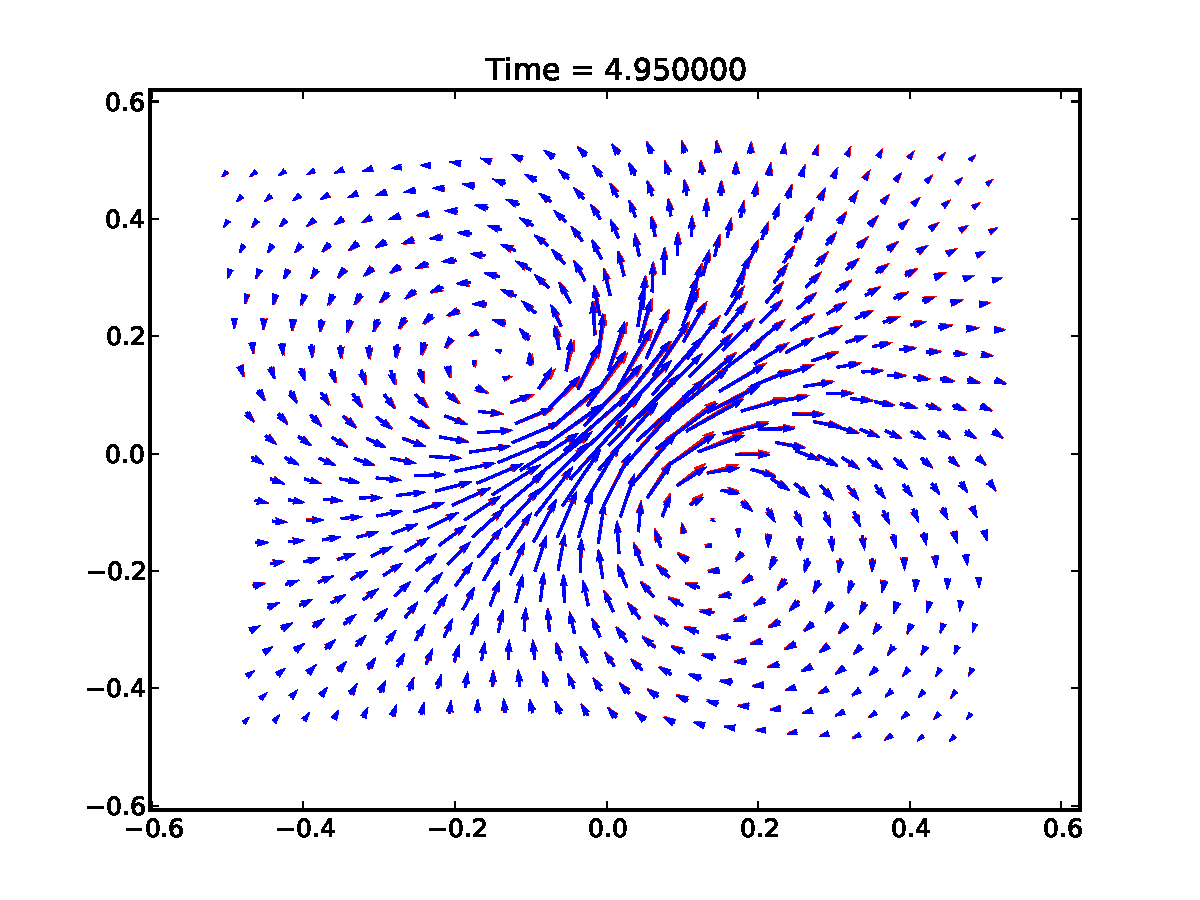
\includegraphics[width=3.5in]{quivframe099.pdf} & 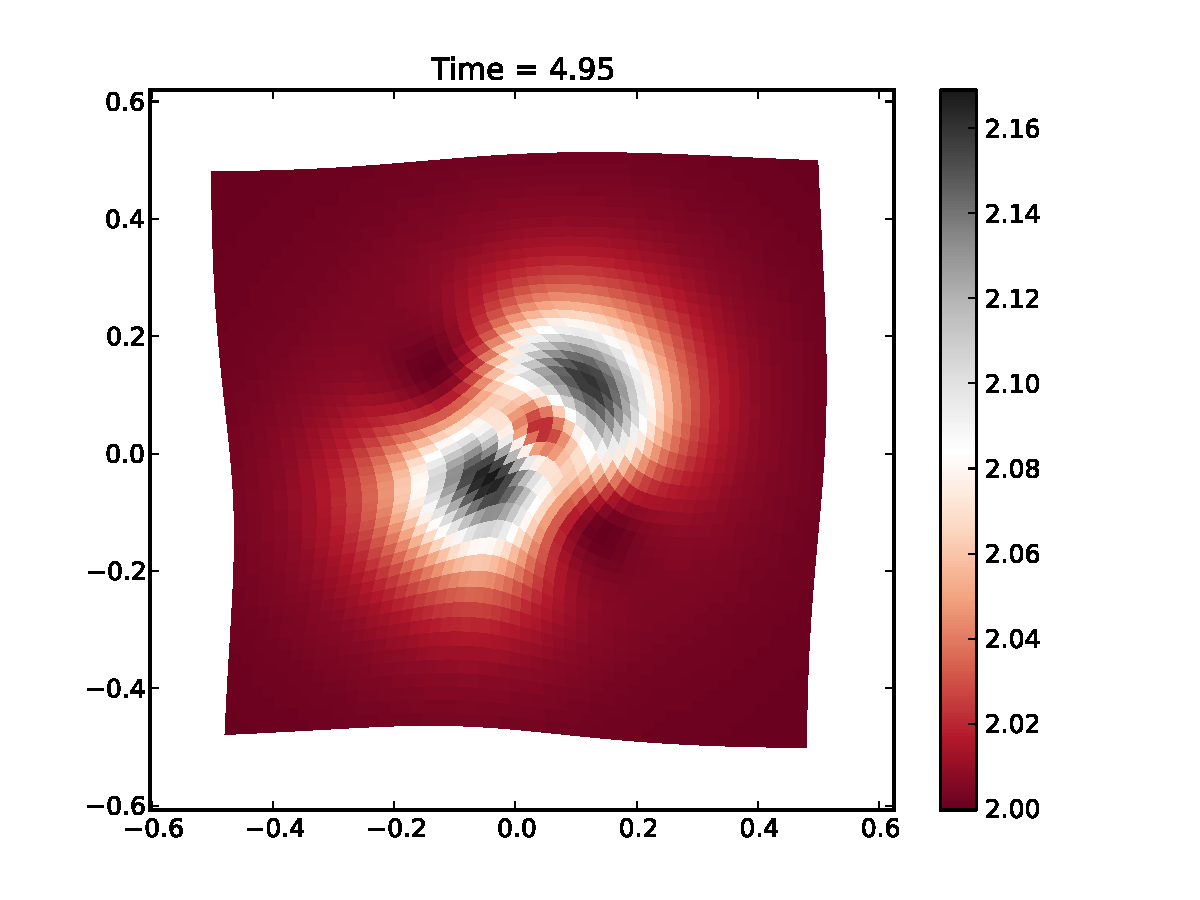
\includegraphics[width=3.5in]{noregridframe099.pdf} 
		\end{tabular}
		\caption{Dipole flow in Stokes-OB fluid at time 4.95. Left: Velocity vectors: The red arrows show the dipole in Stokes flow. The blue arrows show the velocity when it is perturbed by the extra stress in the fluid. Right: The trace of the Eulerian stress tensor $S$. Notice the approximate compactness of the flow.}
		\label{dipolevelvec}
	\end{figure}
	
	I also checked regridding visually using this flow field. I ran the same simulation regridding every 1.0 time units. Fig.~\ref{dipolecontour} shows $S_{11}$ at times 1.0 and 2.0 before and after regridding. The biggest changes to the contours occur near the domain edges, where the contours are forced to close. This happens because I assume no deviation of the stress outside of the domain, which will induce an error. This error will be small for a sufficiently large initial domain around the dipole. Notice that the contours that close are close to the relaxed value of 1.0, indicating that the error in this case is probably small. At later regridding times, the changes in the contours are negligible and are not included here. Similar figures occur for $S_{22}$.

	\begin{figure}[htp]
		\centering
		\begin{tabular}{cc}
			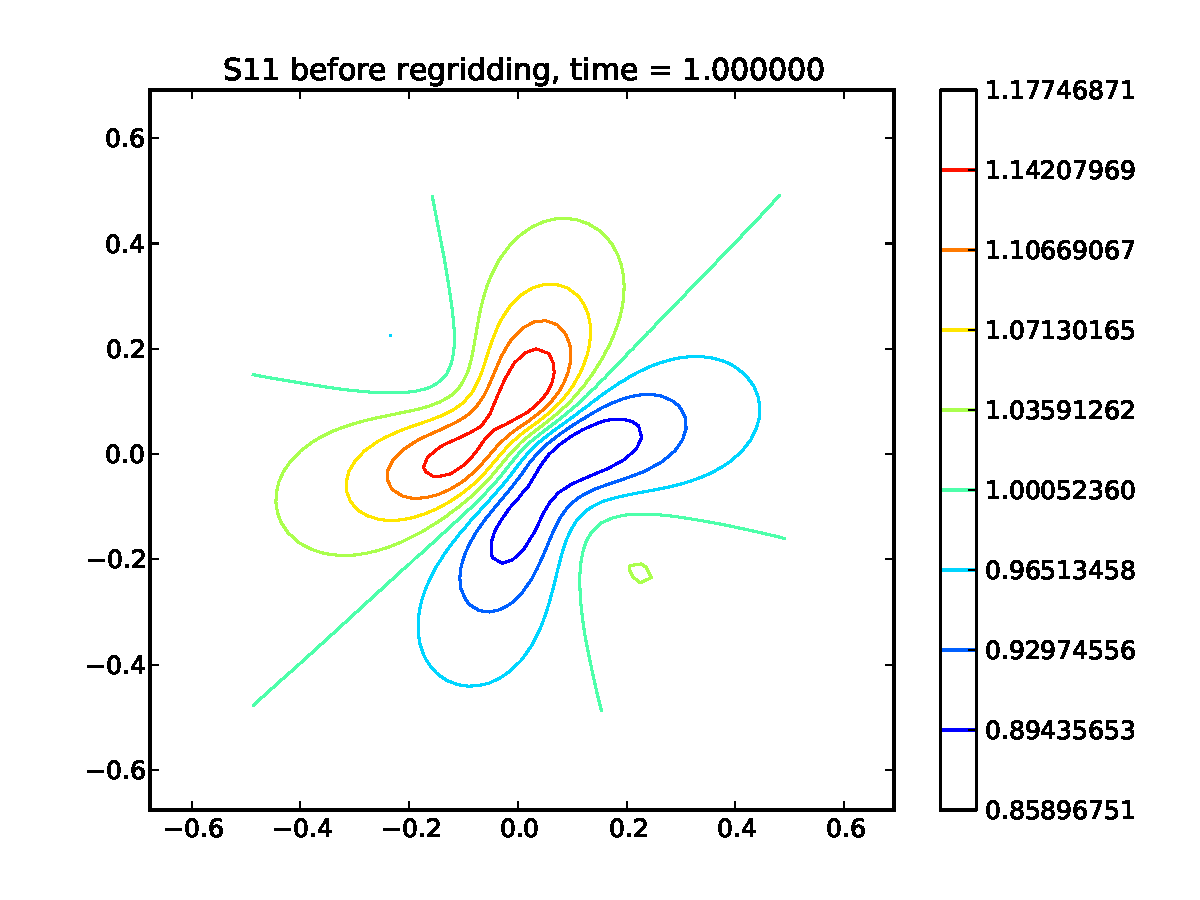
\includegraphics[width=3.5in]{S11Regridding01Before.pdf} & 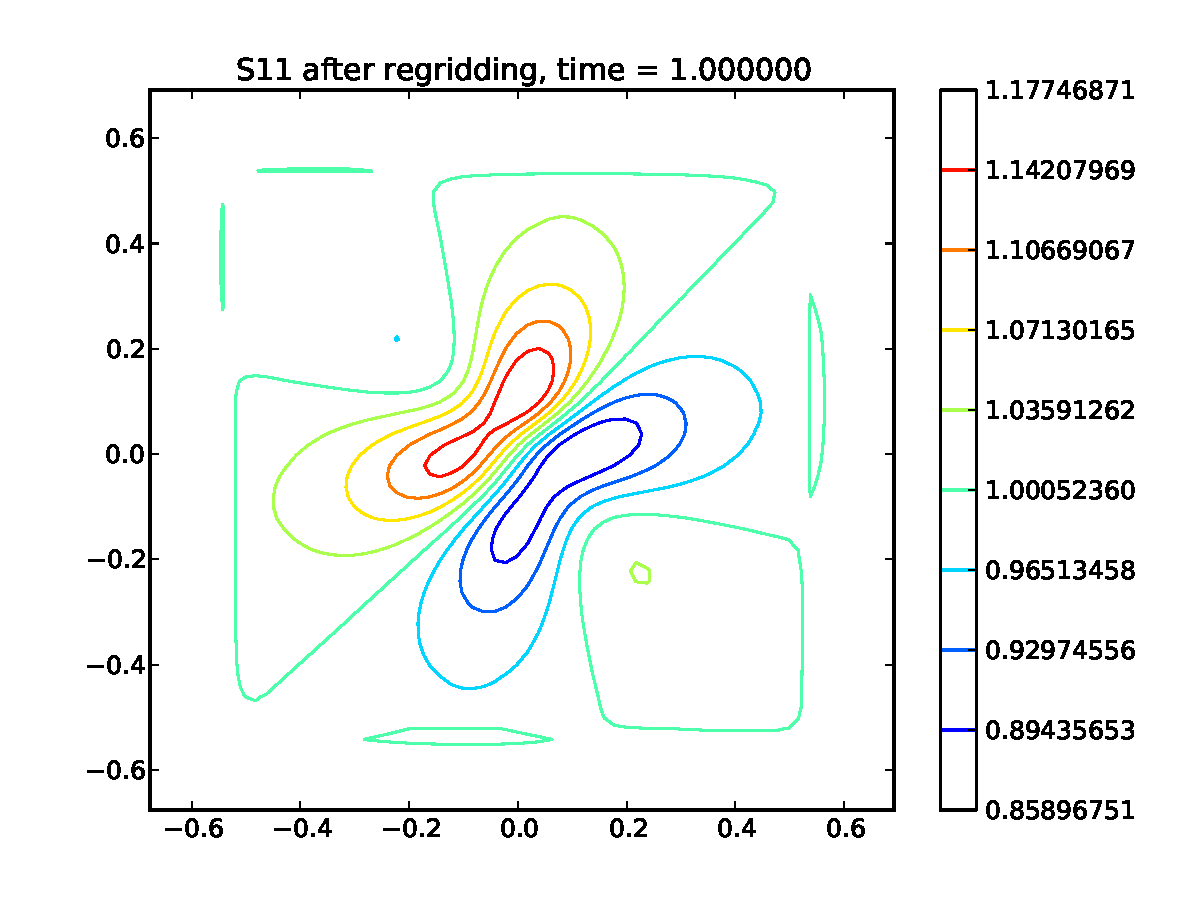
\includegraphics[width=3.5in]{S11Regridding01Regrid.pdf} \\
			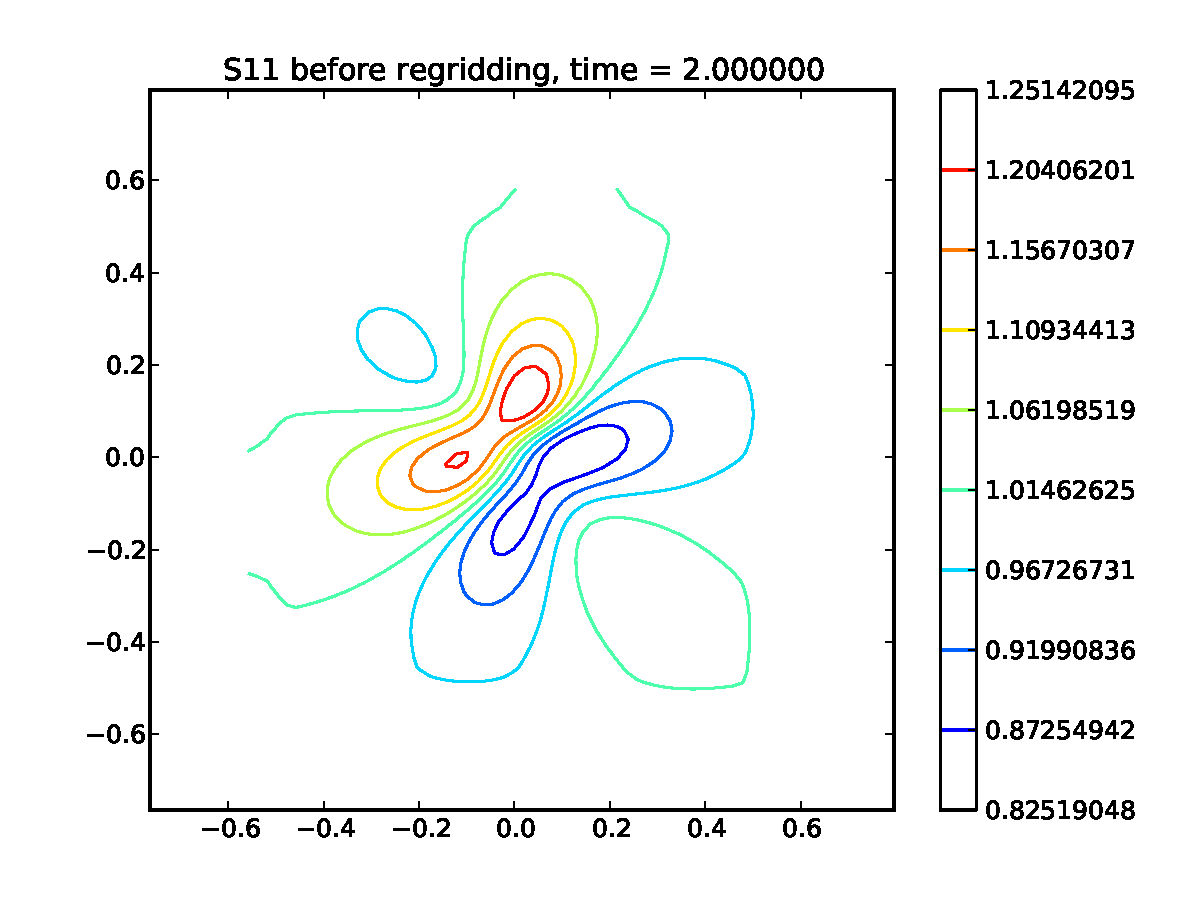
\includegraphics[width=3.5in]{S11Regridding02Before.pdf} & 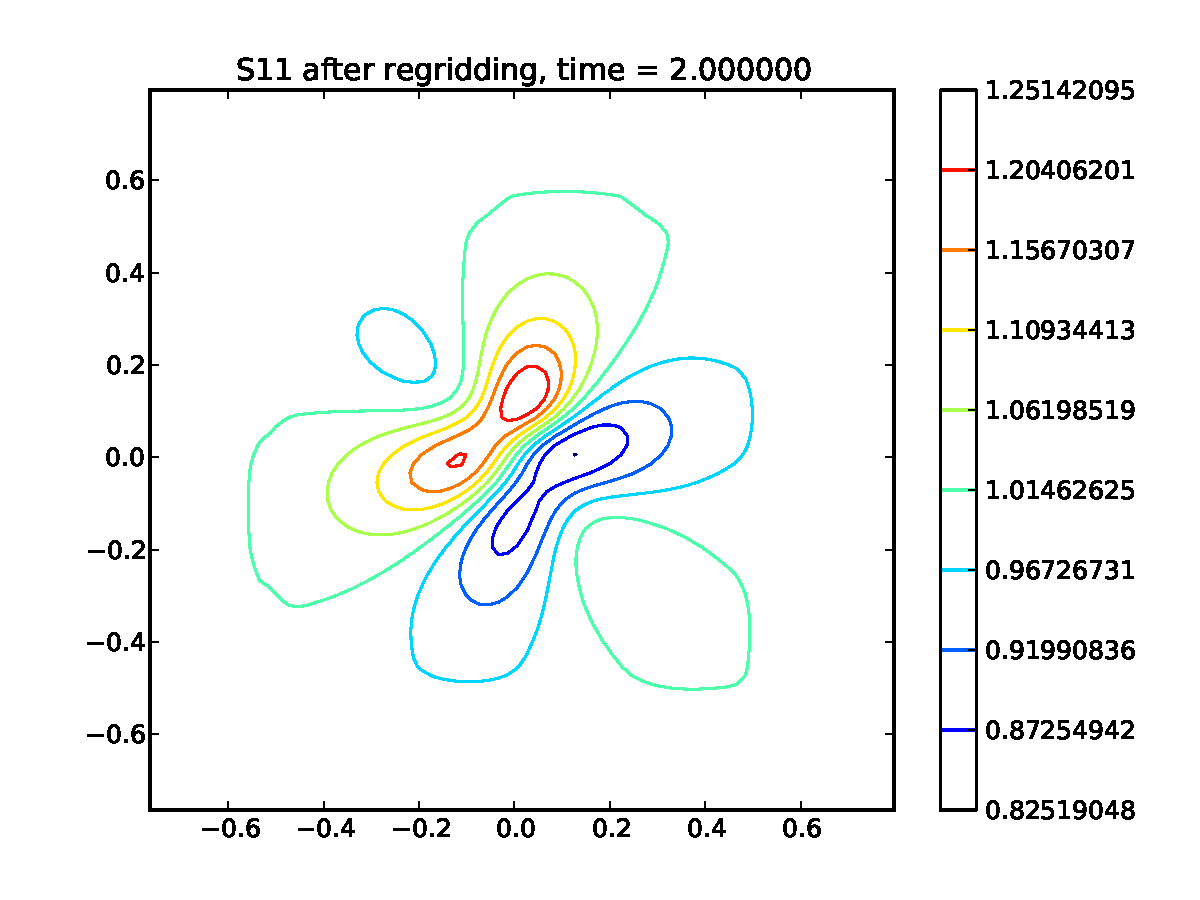
\includegraphics[width=3.5in]{S11Regridding02Regrid.pdf} 
		\end{tabular}
		\caption{Regridding $S_{11}$ for dipole flow at times 1.0 (top row) and 2.0 (bottom row). Left: Contours of $S_{11}$ before regridding. Right: After regridding. Note that the contour lines are forced to close after regridding.}
		\label{dipolecontour}
	\end{figure}
	
	\newpage
	
	\subsection*{Rotating flow}
	
	Next I tried looking at a rotating flow that decays away from the origin:
	%
	\begin{align*}
		\bu_b(x,y) &= Ue^{-r^2}\begin{pmatrix} -y \\ x \end{pmatrix},
	\end{align*}
	%
	where again I write $\bl_0 = (x,y)$ and $r^2 = x^2 + y^2$. By transforming the flow into polar coordinates, it is easy to solve Eq.~\eqref{perturbl}:
	%
	\begin{align*}
		\begin{pmatrix} \dot{x} \\ \dot{y} \end{pmatrix} &= Ue^{-r^2}\begin{pmatrix} -y \\ x \end{pmatrix} \\
			\Rightarrow \begin{pmatrix} \dot{r} \\ \dot{\theta} \end{pmatrix} &= \begin{pmatrix} 0 \\ Ue^{-r^2} \end{pmatrix} \\
			\Rightarrow \begin{pmatrix} x \\ y \end{pmatrix} &= \begin{pmatrix} r_0\cos(\theta_0 + Ute^{-r_0^2}) \\ r_0\cos(\theta_0 + Ute^{-r_0^2}) \end{pmatrix} \\
			\Rightarrow \begin{pmatrix} x \\ y \end{pmatrix} &= \begin{pmatrix} a\cos(Ute^{-a^2-b^2})-b\sin(Ute^{-a^2-b^2}) \\ b\cos(Ute^{-a^2-b^2})+a\sin(Ute^{-a^2-b^2}) \end{pmatrix},
	\end{align*}
	%
	where $r_0,\theta_0$ are the polar Lagrangian coordinates (initial coordinates). The Cartesian Lagrangian coordinates $a,b$ are defined as usual by $r_0^2 = a^2 + b^2$ and $\tan \theta = b/a$.
	
	However I can't solve Eq.~\eqref{perturbP} for $\bP_0$ with $\nabla \bu_b$ and $F = \nabla_a \bl = \begin{pmatrix} \partial x/\partial a & \partial x/\partial b \\ \partial y/\partial a & \partial y/\partial b \end{pmatrix}$ given by the rotating flow. I also tried looking at the Eulerian equations for $\bS$ using the method of characteristics, but this gives a nonhomogeneous, nonconstant-coefficient system that I could not solve either:
	%
	\begin{align*}
		\bS^\nabla &= -Wi^{-1}(\bS - I) \\
		\Rightarrow \pd{\bS}{t} + \dot{x}(t)\pd{\bS}{x} + \dot{y}(t)\pd{\bS}{y} &\equiv \frac{d\bS}{dt} = \nabla\bu_b\bS + \bS\nabla\bu_b^T -Wi^{-1}(\bS - I).
	\end{align*}
	%
	
	There is a worse problem with this flow however: it does not satisfy the Stokes equations. It is clearly an incompressible flow, but there is no pressure gradient that can balance the Laplacian:
	%
	\begin{align*}
		\begin{pmatrix} \pd{p}{x} \\ \pd{p}{y} \end{pmatrix} &= \begin{pmatrix} \nabla^2 u \\ \nabla^2 v \end{pmatrix} = 4U(r^2 - 2)e^{-r^2}\begin{pmatrix} -y \\ x \end{pmatrix} \\
			\Rightarrow \begin{pmatrix} p \\ p \end{pmatrix} &= Ue^{-r^2}\begin{pmatrix} -y(-2x + e^{x^2}(2y^2-3)\sqrt{\pi}\mbox{erf}(x)) + f(y)\\ x(-2y + e^{y^2}(2x^2-3)\sqrt{\pi}\mbox{erf}(y)) + g(x)\end{pmatrix}.
	\end{align*}
	%
	It is easy to see that there is no function $p$ that can satisfy both of these equations.
	
	It is worth noting that Oldroyd (1950) found a rotating solution to the Oldroyd-B model, but it was rotating flow between two cylinders and requires the use of polar coordinates. It would require a reformulation of my code to handle polar coordinates, and is therefore not a good choice for code validation. 
	 
	\subsection*{Parabolic flow}
	
	Here is one last failed attempt: 
	%
	\begin{align*}
		\bu_b(x,y) &= U\begin{pmatrix} xy \\ -\frac{y^2}{2} \end{pmatrix},
	\end{align*}
	%
	which is clearly incompressible. It also satisfies the Stokes equations with an associated pressure of $p = -U\mu y$. Furthermore, Eq.~\eqref{perturbl} can be solved easily since the ODEs are separable to get 
	%
	\begin{align*}
		x &= \frac{x_0y_0^2}{4}\left(Ut+\frac{2}{y_0}\right)^2 \\
		y &= \frac{2y_0}{Uy_0t+2},
	\end{align*}
	%
	where $(x_0,y_0)$ are the initial conditions and Lagrangian variables. The Eulerian equations for the stress using the method of characteristics separate nicely:
	%
	\begin{align*}
		\frac{dS_{11}}{dt} &= \left(2Uy - \frac{1}{Wi}\right)S_{11} + 2UxS_{12} + \frac{1}{Wi}\\
		\frac{dS_{12}}{dt} &= 2- \frac{1}{Wi}S_{12} + UxS_{22}\\
		S_{21} &= S_{12} \\
		\frac{dS_{22}}{dt} &= \left(-2Uy - \frac{1}{Wi}\right)S_{11} + \frac{1}{Wi},
	\end{align*}
	%
	so that one can solve for $S_{22}$, $S_{12}$, and $S_11$ in order after substituting in the expression for $y(t)$. I was able to solve for $S_22$ in Mathematica, but not for $S_{12}$ afterwards. And furthermore, it looks like this flow might not have compact stress. So I gave up.
	
	
	
	
	
	
	
	
	
	
	
	
	
	
	


\end{document}